\documentclass[twoside,11pt]{article}

% Any additional packages needed should be included after jmlr2e.
% Note that jmlr2e.sty includes epsfig, amssymb, natbib and graphicx,
% and defines many common macros, such as 'proof' and 'example'.
%
% It also sets the bibliographystyle to plainnat; for more information on
% natbib citation styles, see the natbib documentation, a copy of which
% is archived at http://www.jmlr.org/format/natbib.pdf

\usepackage{jmlr2e}

\usepackage{float}
\usepackage{caption}
\usepackage{subcaption}
\usepackage{tabularx}
\usepackage{graphicx}
\usepackage{framed}
% Definitions of handy macros can go here

\newcommand{\dataset}{{\cal D}}
\newcommand{\fracpartial}[2]{\frac{\partial #1}{\partial  #2}}

\newenvironment{changemargin}[2]{%
\begin{list}{}{%
\setlength{\topsep}{0pt}%
\setlength{\leftmargin}{#1}%
\setlength{\rightmargin}{#2}%
\setlength{\listparindent}{\parindent}%
\setlength{\itemindent}{\parindent}%
\setlength{\parsep}{\parskip}%
}%
\item[]}{\end{list}}

% Heading arguments are {volume}{year}{pages}{submitted}{published}{author-full-names}

%\jmlrheading{1}{2000}{1-48}{4/00}{10/00}{meila00a}{Marina Meil\u{a} and Michael I. Jordan}

% Short headings should be running head and authors last names

\ShortHeadings{Railway Signalling and Delay Estimation via Simulation}{Arjun}
\firstpageno{1}

\begin{document}

\title{Railway Signalling and Delay Estimation via Simulation}

\author{\name Arjun Krishna \email ark@cse.iitm.ac.in \\
       \addr Department of Computer Science and Engineering\\
       Indian Institute of Technology, Madras\\}

\editor{}

\maketitle

\begin{abstract}%   <- trailing '%' for backward compatibility of .sty file

\end{abstract}
	The paper describes a method for delay estimation and congestion estimation in the railway 
	network using simulations.
	The key idea is to model the railway network as a computer network with
	various stations being nodes and trains being packets and run a Discrete Event
	Simulator SimJava with well defined signalling protocols to observe 
	some useful statistics.
	In this paper simulations are run on the static schedule of the Southern Indian railways; a dataset curated by scraping the indiarailinfo site.
	The simulations results in statistics about delays at various nodes and contention 
	for a particular link in the network indicating congestion in the network.
	
	The simulation results for schedule improvements are presented using the 
	$O$(congestion + dilation) packet routing described by Leighton, Maggs and Rao \cite{LMR} and also present a schedule improvement strategy which
	introduces small delays at some intermediate stations than just delay at source.  \\
	
\begin{keywords}
  Discrete event simulation (SimJava) , Delay estimation, Congestion estimation, 
  O(congestion + dilation) packet routing
\end{keywords}

\section{Introduction}

Train Delay is the measure of deviation from the fixed schedule of the train, 
the delays can occur due to a variety of reasons like signalling delays, train interference etc., some of these reasons are controlled by the railway operators
and some others indeterminable. The goal of the paper is to present a simulation
method for estimating the train delays assuming a approximate model of how 
the railways actually performs. \\ 

Simulation methods are very useful when it is very hard to estimate some variables analytically. In the literature for delay estimation there has been a lot of analytical, history data based and simulation methods. The simulation method is apt for this setting as the railway network is a very complex entity and via simulations one can attempt to model the complex network as close as possible without a lot of relaxations, thereby enabling us to estimate the variables accurately. \\


\indent Train Delay estimation plays an important role in railway optimizations, as it
gives a better knowledge of the system and various factors that cause delays so
enabling the railway operators to strategize and operate efficiently. The paper
discusses some simple signalling protocols that are used by the railways and
modelling them as a computer network protocol, enabling the use of discrete-time
simulator SimJava to run simulations under certain assumptions of train speed, 
signal placement etc., to estimate the delays caused at various nodes. \\

The network simulation is run for a fixed schedule of the Southern Indian Railways which is curated by scraping the indiarailinfo site. The simulation is run for a weekly schedule, however this can be easily extended based on the computational resource available. The simulation logs the delay faced by a train at a particular node and also if there is contention it logs the array of trains contending for a link. This log is analysed to present the results in this paper, which gives a fair indication of how the schedule performs. \\


Schedule improvement can be done via the $O$(congestion + dilation) suggested by Leighton, Maggs and Rao \cite{LMR}, where all the trains are delayed at the source by a random amount of time.
It is empirically observed that there is a significant reduction in average delay at a node and the average end-to-end delay a train faces. Also, it is shown that instead of an initial delay at the source of the train, a similar performance output can be obtained by performing small delays at random nodes on the path of the train.


\section{Railway Signalling Protocols}

Railway Signalling Protocols ensure rail safety and control railway traffic.
The protocols dictate how the train has to travel between two stations.
There are two main types of signalling methods \vspace{0.2in} \\
{\bf Time Interval Method :} The trains are spread over the length of the track
in such a manner that if the train ahead stops, the following train would be 
able to stop without collision. This methods works if the traffic is less and
would be risky when considering passenger trains. \\
{\bf Space Interval Method :} In this method the track is divided into 
blocks, the protocol ensures that a train can enter a block only if there is
no other train in that block.\\

{\noindent \underline{ \bf Signalling Systems }}  \vspace{0.05in} 

{\noindent \bf Semaphore Signal :} This was the earliest form of fixed railway 
signal, the information is conveyed to the locomotive driver from the inclination
of the pivoted arm on a vertical post. This was the widely used form of mechanical
signalling. Colour Light signals have replaced most of these Semaphore Signals today.
\begin{center}
	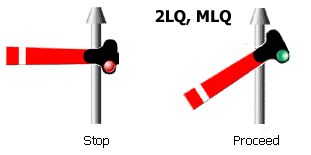
\includegraphics[scale=0.5]{img/2lq.png} \\
	\textbf{Figure 1:} Semaphore Signal  
\end{center}

{\noindent \bf Colour Light Signals : } In this system colour lights are used to 
convey information to the train driver, the key advantage over Semaphore signal is 
that it is visible over longer ranges and there is no mechanical movements involved.

\begin{center}
	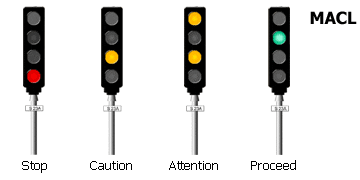
\includegraphics[scale=0.6]{img/macl.png} \\
	\textbf{Figure 2:} Colour Light Signal 
\end{center}

The red signal indicating the train has to stop before moving to the next
block. The green signal indicating that the train has acquired permission to
proceed further. A single yellow (caution) conveys to the train driver 
to proceed and be prepared to stop at the next block. A double yellow signal (attention) conveys to the locomotive driver to pass the next signal at a 	restricted speed. \\
\indent These protocols ensure that any two trains are never in the same block. In this paper the above protocols are modelled as a computer network protocol to enable us to simulate the train movement using the SimJava simulator running the Signalling Protocol.

\section{Protocol for Modelled Railway Network}

\underline{\bf Modelling the Semaphore Signals } \vspace{0.1in} \\
The Semaphore Lock Signal is modelled with the following event based algorithm. This is the protocol on which the simulation results are based on. The image below is a visual depiction of the protocol. 
\begin{center}
	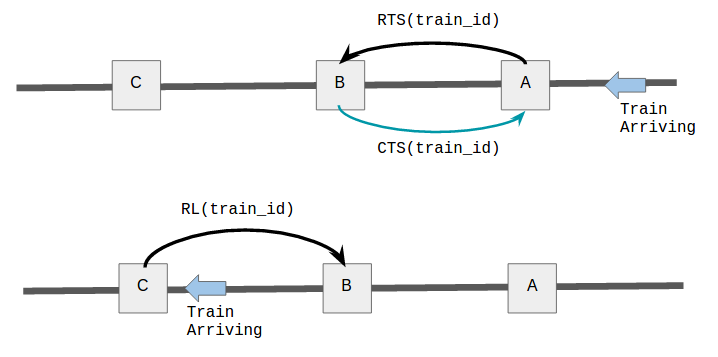
\includegraphics[scale=0.46]{img/semaphore_protocol.png} \\
	{\bf Figure 3:} Semaphore Signal based protocol visualization  \\ \vspace{0.05in}
	{\bf RTS :} {\em Request To Send} $|$
{\bf CTS :} { \em Clear To Send} $|$
{\bf RL  :} { \em Release Lock  }
\end{center}

\newpage
\noindent \underline{ SIGNALLING PROTOCOL }
\begin{framed}
\begin{itemize}

	\item {\bf Event } : Train Packet Received \\
		  {\bf Action }: 
			\begin{itemize}
				\item Send RL (train\_id) to the previous node in the route.
				\item Send RTS (train\_id) to the next node in the route. 
				\item Store the packet in the buffer.
			\end{itemize}
			
	\item {\bf Event } : RTS (train\_id)  \\
		  {\bf Action }: \\
		  \begin{framed}
		  	\underline{Definition}
	\begin{itemize}
	\item if node is a STATION, then L is a Semaphore Lock with maximum count being number of platforms.\\ $ M = $ platform\_count
	
	\item if node is a SIGNALLING NODE, then L is a binary Semaphore Lock. \\ $ M = 1 $
\end{itemize}
	\end{framed}
    {\bf if} ( L $ < M $)  : \\
     \indent \hspace{0.1in}   acquire(L) \\
     \indent \hspace{0.1in}   Send CTS(train\_id) to the requesting Node. \\
    {\bf else} : \\
	\indent \hspace{0.1in}   Buffer RTS packet in requesters queue. 

	\item {\bf Event } : CTS (train\_id) \\
		  {\bf Action }:	 
	\begin{itemize}
		\item Send the buffered train packet identified by train\_id to the next node. 
	\end{itemize}

	\item {\bf Event } : RL (train\_id) \\
		  {\bf Action }: \\
		  
	{\bf if}  ( requesters.empty() ) : \\
	 \indent \hspace{0.1in}     release(L) \\
	 \indent \hspace{0.1in}   clear all train\_id related storage in buffers. \\
	{\bf else} : \\
	 \indent \hspace{0.1in} Pop the RTS packet from queue \\
     \indent \hspace{0.1in} Send CTS (train\_id) based on the RTS packet to the requester. \\


\end{itemize}
\end{framed}


\noindent\underline{\bf Modelling the Colour Light Signals  } \vspace{0.1in} \\
Each signalling unit is a node in the modelled network and has a lock associated
with it, a train that acquires this lock will be granted permission to move on
to the next signal. \\
If the train is reaching a signalling node {\em A}, The node {\em A} anticipates this and would send a message to the next signalling node on the track, say {\em B}, and the node next to {\em B} say {\em C}. If the lock at node {\em B} is acquired then the signal at {\em A} is red, else If the lock at {\em C} is not acquired then the signal at 
node {\em A} is green, allowing the train to proceed further. If it is acquired then 
the signal would be yellow. \\

\begin{center}
	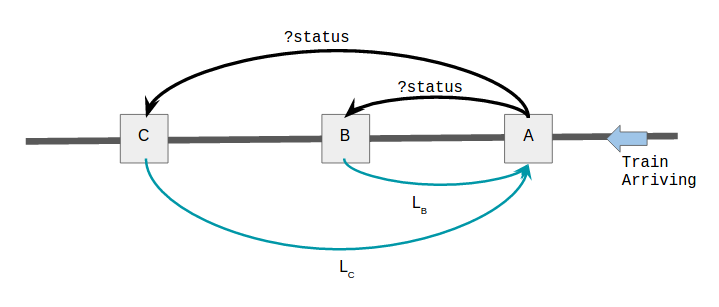
\includegraphics[scale=0.5]{img/signalling.png} \\
	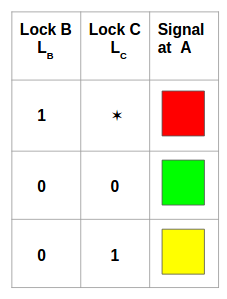
\includegraphics[scale=0.5]{img/signalling-chart.png} \\
	{\bf Figure 4:} Signalling protocol based on the Colour Light Mechanism  \\
	{\em ( Lock is 1 if it is acquired by some other train already )}
	
\end{center}

If the train is signalled red, then it waits at that block until
the next block sends a message that it's lock is free. The signalling element is 
designed such that whenever permission for a train to acquire the lock is denied the
event is logged and the requester gets a clearance once the lock is available. \\

	Through this protocol train speed can be varied based on observed signal eg. if the train sees an yellow signal the packet speed can be decreased. Also speed can be varied based on the history of signals seen by the train. This protocol is fairly complex and is a part of the future work, the simulation results are obtained using the Semaphore based signalling scheme.
 
\newpage
 
\section{Train Delay Estimation}

The train delay is the measure of deviation from the schedule, it is quite 
important to record these train delays or estimate them so that railway operations 
can be more efficient, with appropriate strategies developed to tackle delays. \\

There are a lot of reasons for delays to occurs in the railway operations some of them
are listed below 
\begin{itemize}
	\item \underline{ Track and Signal Delays} : caused due to track maintenance or signals that ensure reduced speeds for safe operation.
	\item \underline{ Train Interference Delays} : caused due to other trains in the
	route, includes delay caused in switching tracks. 
	\item \underline{ Equipment Delays} : caused predominantly due to equipment failure or unscheduled maintenance.
	\item \underline{ Weather Delays} : caused due to the weather condition.
	\item \underline{ Passenger Delays } : accounts for the waiting time for passenger boarding and de-boarding, and delays in passenger service.
	\item \underline{ Operational Delays} : Delays due to crews operation of the train, such as delay in the starting of the train, detour etc.,
\end{itemize}

Though some factors like Signal Delays, Train Interference Delays can be obtained by direct simulations, the other delay factors have to modelled as
probability distributions based on historical data to include them in the simulation. Train delay estimation is an important problem and documenting delays at various parts of the network would be useful for the railway operations to strategize better. There are three widely studied techniques for train delay estimation in the literature: Analytical Method, Data-based Approach, Simulation. \\

{\noindent \bf Analytical Method }  \\

In this method the railway network is mathematically modelled, assuming
a few parameters of the network and provide a probabilistic model of the trains.
Using the mathematical formulation delay estimates can be obtained. Though,
it is possible to get a clear mathematical formulations, it is hard to capture a variety of complex
interactions between the trains and some initial mathematical assumptions might
not be realistic. Hence, Analytical Methods do not capture the real-life complex
interactions in the railway network, thus would not provide good delay estimates.  \\

{\noindent \bf Data-based Approaches } \\

With the availability of a lot of historic data about train journeys, Data-based
approach of delay estimation is very practical and provides good estimates. This
allows to consider various parameters that determine delay on a network and build
a regression model with these features and the train travel records to perform
delay estimation. These models can also help in identifying important features
that cause a lot of delay. The major drawback of this method is that there is 
no sufficient data available on the Indian Railways operation and hence the data based approach would be hard to apply.
\\

{\noindent \bf Simulation methods} \\

Simulation methods actually simulate the railway network in-order to extract
actual train performance and delays. The simulations gives scope to handle various parameters of the network and hence can model the task on hand with flexibility and 
produce fairly accurate delay estimates. The simulated methods can embed a
lot of complex interactions that are analytically hard to conceptualize and with
a properly tuning of parameters the train delay statistics are easily obtained. Simulation models are intuitively good for delay estimation but it is still an approximation to the actual railway operation because it is very hard to capture all the complex features of operation. \\

In this paper a discrete time simulation model for the Railway Network ( modelled as computer network) using SimJava is presented. The presented Network model simulates a static timetable of the Southern Indian Railway Schedule obtained by scraping the indiarailinfo website. The model runs the Semaphore based Signalling protocol, and the delay a train occurs at a node is the time delay in getting a CTS packet once an RTS packet is fired, this delay is logged. Any contention for accessing a block is identified when buffering requesters and this is also logged as it directly indicates the congestion in the network.  

\section{O(congestion + dilation) packet routing}

O(congestion + dilation) is the best one can do when it comes to packet routing, as both the factors act as a lower bound and have a grip on the end-to-end routing time. Leighton, Maggs and Rao \cite{LMR} prove that it is possible to produce a O(congestion + dilation) schedule for routing.

The following online algorithm which does a random delay at the source of the train is adopted from Leighton, Maggs and Rao. Following are a few definitions after which the algorithm used is presented, for proofs please refer to the paper. \\

\noindent \underline{\emph{Definition :}}
\begin{enumerate}
	\item Dilation $d$, is the longest routing path on the network. This is an obvious lower bound on the total routing time
	\item Congestion $c$, is the maximum of the number of routing path crossing a edge.
\end{enumerate}

\noindent \underline{\em Parameters :} 

\begin{itemize}
	\item Let $c$ be the congestion in the network
	\item Let $N$ be the number of packets.
	\item Let $d$ be the dilation of the network.
	\item Let $\alpha$ be a constant.
\end{itemize}
\noindent The following algorithm provides an $O(c + d \log(N d))$ length schedule. It produces near optimal schedule for high $c$, though this is not the case in the Railway Network, schedule improvements using the following technique is observed experimentally.\\

\underline{\bf Randomized on-line algorithm}
\begin{framed}
\begin{enumerate}
\item Each packet is assigned a delay chosen randomly, independently and uniformly
	  from the interval $ [ 1 , \frac{\alpha c}{\log(N d)} ] $
\item The packet waits for delay chosen at source, and is routed without stopping.
\end{enumerate}
\end{framed} 
\hrule 
\vspace{0.1in}
\noindent The following procedure produces a $O((c+d)2^{O(\log^*(c+d))})$ length schedule. \\

\noindent \underline{\em Definition :}
\begin{enumerate}
\item A frame is a sequence of T time steps
\item Congestion of a frame, C is the maximum number of packets crossing any edge in the frame
\end{enumerate}

\noindent {\bf Lemma :} For every set of packets that has congestion $c$ and dilation $d$, there exists a schedule of length $O(c + d)$ such that no packet ever waits in queues once it starts and the relative congestion of any frame of length less than $\log d$, is at most $1$. \\

In the lemma, a schedule is created by the randomized on-line algorithm, which is used to recursively build a schedule to obtain the desired $O((c+d)2^{O(\log^*(c+d))})$ length schedule, which is done as follows.

\begin{enumerate}
\item By using Lemma, produce a schedule S where the number of packets that use an edge in any frame of length $\log d$ is at most $\log d$.
\item Break the schedule into frames of size $\log d$.
\item Consider each frame of length $\log d$ as a new routing problem that has dilation and congestion $\log d$, and solve it recursively, until the frames have constant size and at most a constant number of packets use each edge in each frame.
\end{enumerate}
\hrule 
\vspace{0.1in}

\noindent The choice of the parameter $\alpha$ should be quite high to be effective, but it also indicates the maximum delay that can be inflicted in the schedule. Results are obtained for simulations done using the randomized on-line algorithm provided by LMR. \\


The following is another alternative algorithm which unlike the randomized on-line algorithm that inflicts random delays at the source, induces smaller random delays at random intermediate nodes on the route of the packet. In this case a frame is defined to be the subset of nodes in the route of the packet whose size is less than a fixed length $L$. Let $\beta$ be a fixed constant, which is similar to parameter $\alpha$ but would be lower. \\

\underline{\bf Random Delay at Intermediate Nodes }
\begin{framed}
\begin{enumerate}
\item For each packet assign a source delay randomly chosen in the interval $ [ 1 , \frac{\beta c}{\log(N d)} ] $ 
\item As the packet is routed in its assigned path, with a probability p = $\frac{1}{L}$ pick a random delay in the interval $ [ 1 , \frac{\beta c}{\log(N d)} ] $ for a node in the path.
\end{enumerate}
\end{framed}
It is empirically observed that the above algorithm like LMR offers a significant reduction in end-to-end delays, and the frequency of seeing large delays.

\section{Results}

The modelled Network simulation is run on the Southern Indian Railway Schedule. 
The following are the details of the network
\begin{itemize}
\setlength\itemsep{0.1cm}
\item Number of stations              :  565
\item Number of Signalling Nodes      :  10766
\item Dilation (d)                    :  356
\item Number to trains Scheduled (N) :  2712
\end{itemize}
The time measured in simulation is the number of seconds since 00:00 AM, Monday. Using this base line all the departure timing of the train is converted to simulator time in-order to schedule it accordingly. \\

\noindent The result organization is as follows
\begin{itemize}
 \setlength\itemsep{0.1em}
 \item {\bf Default :} Simulations run with default parameters as specified by the modelling paper. The congestion $c$ is estimated from this run as it is more realistic than calculating the worst case congestion. Using this $c$ the algorithms described in the previous section are run. It is observed from the data collected that $c = 3$.
  \item {\bf LMR : } Simulations run with train packets randomly delayed at the source as specified by the previous section. The results are presented for the on-line  randomized algorithm with parameter $\alpha=3000$ which dictates the maximum delay at source to be $\frac{\alpha c}{\log (Nd) }$  which turns out to be about 10 min.
  \item {\bf RDIN : } Simulations run with introducing small random delays in some intermediate stations in the path of the train. The results are presented for the Random Delay at Intermediate Nodes algorithm, with $\beta=100$ which indicates that the  delay at an intermediate node is at most 20 seconds ( $\frac{\beta c}{\log (Nd) }$ ) 
\end{itemize} 

\subsection{Default}

\begin{tabular}[htp]{cc}
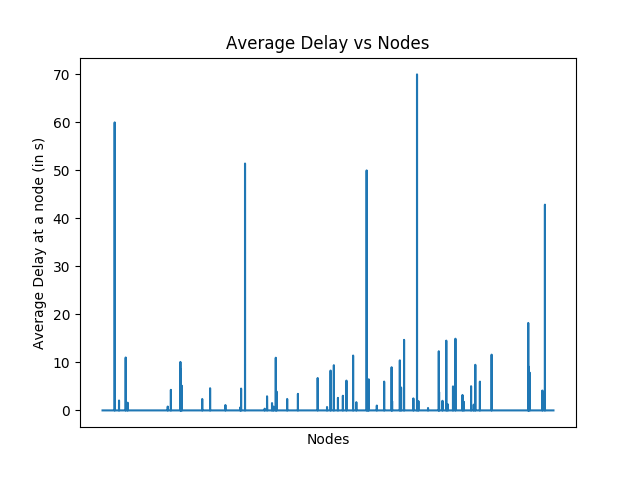
\includegraphics[width=0.45\textwidth]{img/Default/figure_1.png} 
&
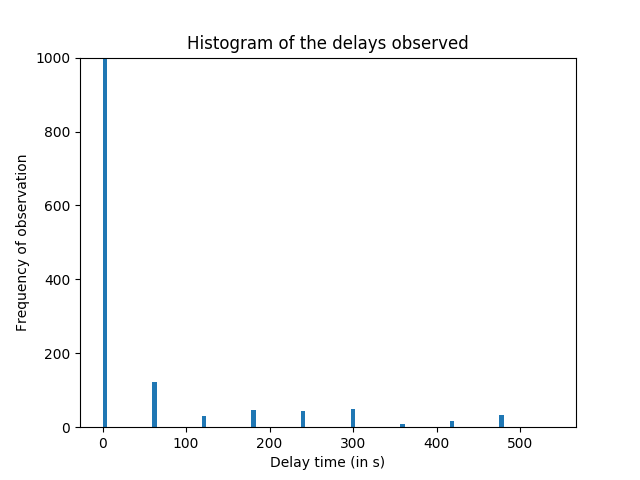
\includegraphics[width=0.45\textwidth]{img/Default/figure_1-1.png} \\

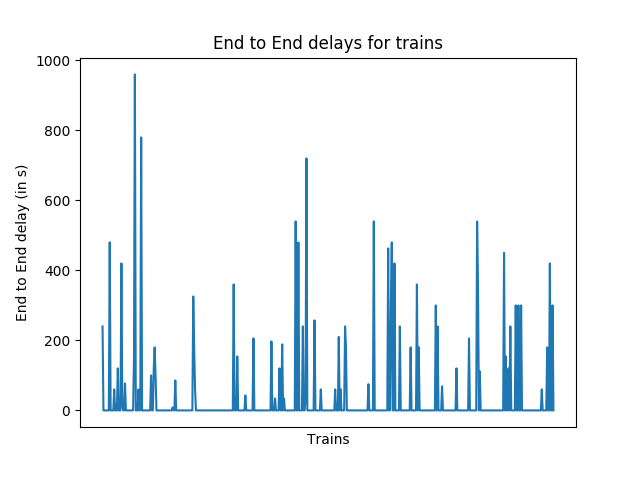
\includegraphics[width=0.45\textwidth]{img/Default/figure_1-2.png} 
&
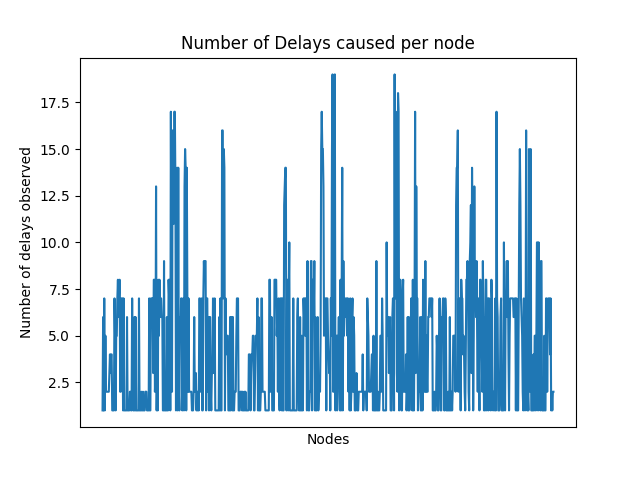
\includegraphics[width=0.45\textwidth]{img/Default/figure_1-3.png}  \\
\\
\multicolumn{2}{p{\textwidth}}{
The above plots indicate the simulation results for the default run of the schedule on the modelled network. The maximum contention observed is 3. The total end-to-end delay is at most 980 seconds ($\approx$ 16 min). In the histogram of delays observed as expected most frequent are the low delays, but some taxing delays of upto 8 minutes are also observed. \newline \newline
The maximum congestion observed $c = 3$ is used as the parameter need in applying the LMR, RDIN schedule improvement procedure.  \vspace{2.5in}}
\end{tabular}

\subsection{LMR}

\begin{tabular}{cc}

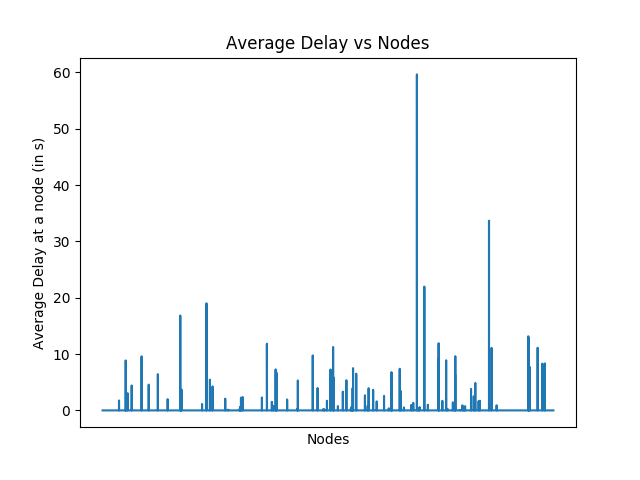
\includegraphics[scale=0.4]{img/LMR/alpha=3000/figure_1.png} 
&
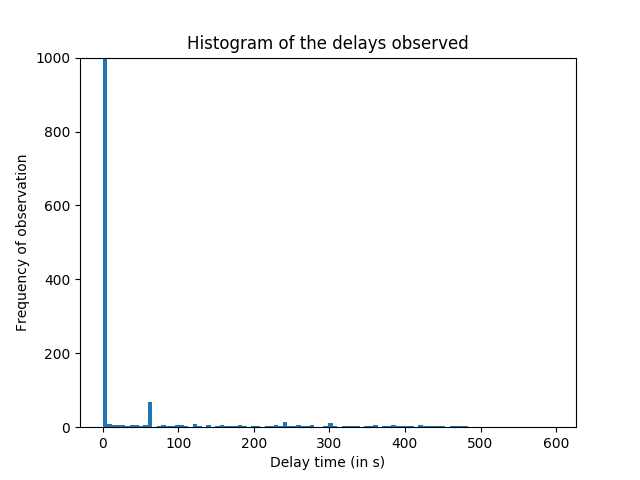
\includegraphics[scale=0.4]{img/LMR/alpha=3000/figure_1-1.png} \\

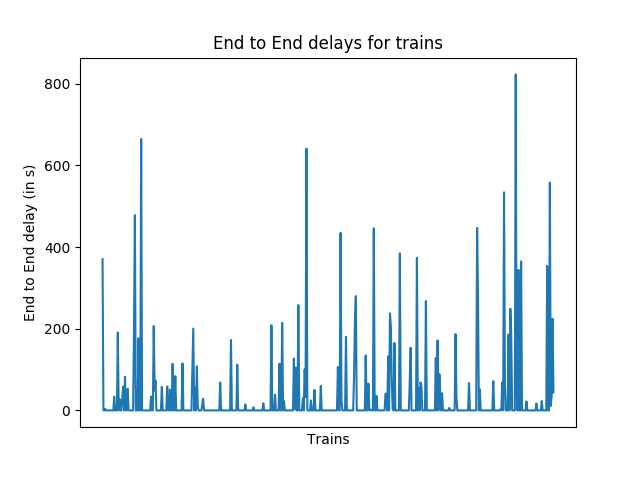
\includegraphics[scale=0.4]{img/LMR/alpha=3000/figure_1-2.png} 
&
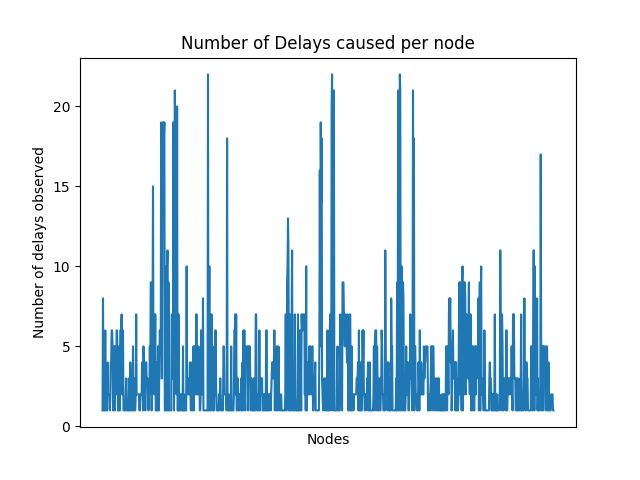
\includegraphics[scale=0.4]{img/LMR/alpha=3000/figure_1-3.png}  \\
\multicolumn{2}{p{\textwidth}}{
The above plots indicate the simulation results for the LMR randomized algorithm applied to the Southern Railway Schedule. The congestion $c = 3$ and parameter $\alpha = 3000$ indicates the maximum a train can get delayed at source is 10 minutes. \newline \newline
A significant reduction of the maximum end-to-end delay of a train is observed,  reducing the maximum delay by around 3 minutes. The average delay that occurs at node is also significantly reduced. The histogram depicts that very large delays occur very rarely even less frequent than the default run. Though the number of delays caused by nodes might have slightly increased, the histogram convinces the fact that the delay caused is probably lower. \newline \newline
Therefore, as expected from theory randomized on-line algorithm presented by Leighton, Maggs and Rao \cite{LMR} offers a significant reduction in major delays that occur due to contention and offer an improved schedule.
\vspace{1.6in}}
\end{tabular}


\subsection{RDIN}

\begin{tabular}{cc}

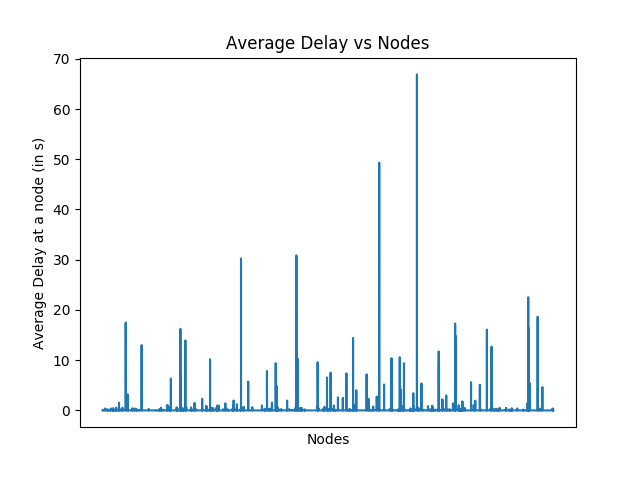
\includegraphics[scale=0.4]{img/IND/figure_1.png} 
&
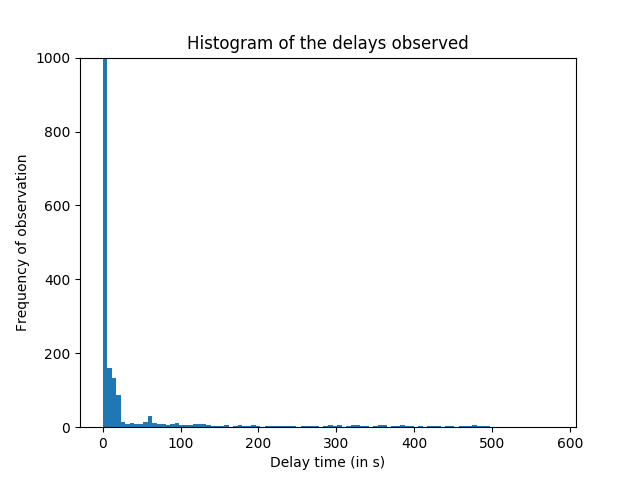
\includegraphics[scale=0.4]{img/IND/figure_1-1.png} \\

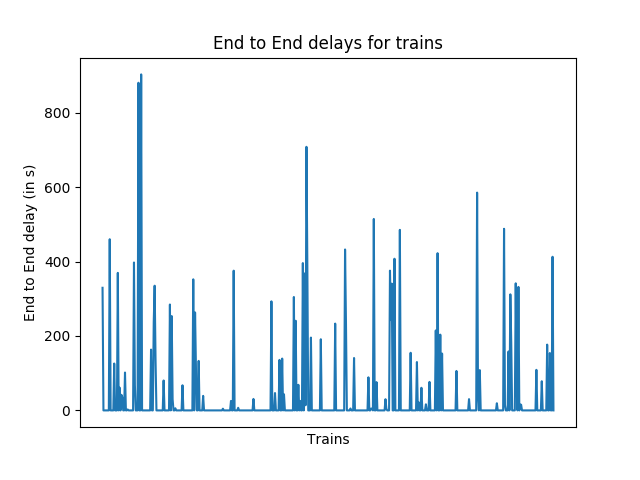
\includegraphics[scale=0.4]{img/IND/figure_1-2.png} 
&
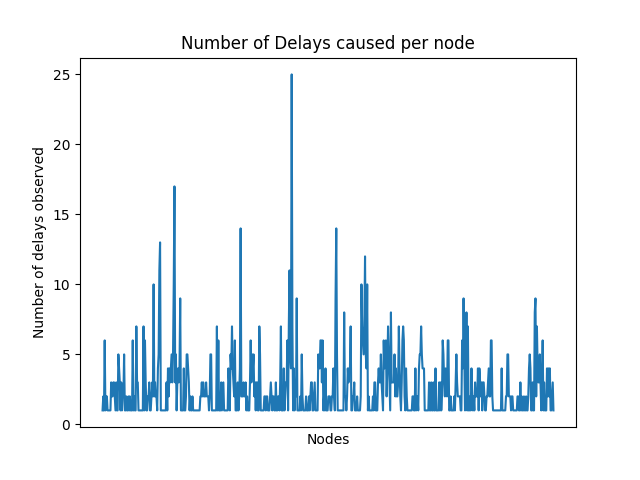
\includegraphics[scale=0.4]{img/IND/figure_1-3.png} \\
\multicolumn{2}{p{\textwidth}}{
The above plots indicate the simulation results for the RDIN algorithm applied to the Southern Railway Schedule. The congestion $c = 3$ and parameter $\beta = 100$ indicates the maximum a train can get delayed at any node on its path is at most 20 seconds.\newline \newline
A significant reduction of the maximum end-to-end delay is observed and is very similar to LMR algorithm. The average delay that occurs at node does not change much. The histogram still indicates that very large delays do not occur as often as the default case, however in performance is slightly poorer than LMR. The number of delays seem to have increased,but since it is rare to see high delays it is presumably very minor delay occurrences. \newline \newline
This method is in fact useful for schedule improvement as it is feasible to induce small train delays at an intermediate stations which brings down the end-to-end delay therefore can be easily incorporated in the schedule.
\vspace{1.6in}}

\end{tabular}


\newpage 
\begin{changemargin}{-3cm}{-3cm}
\begin{center}
	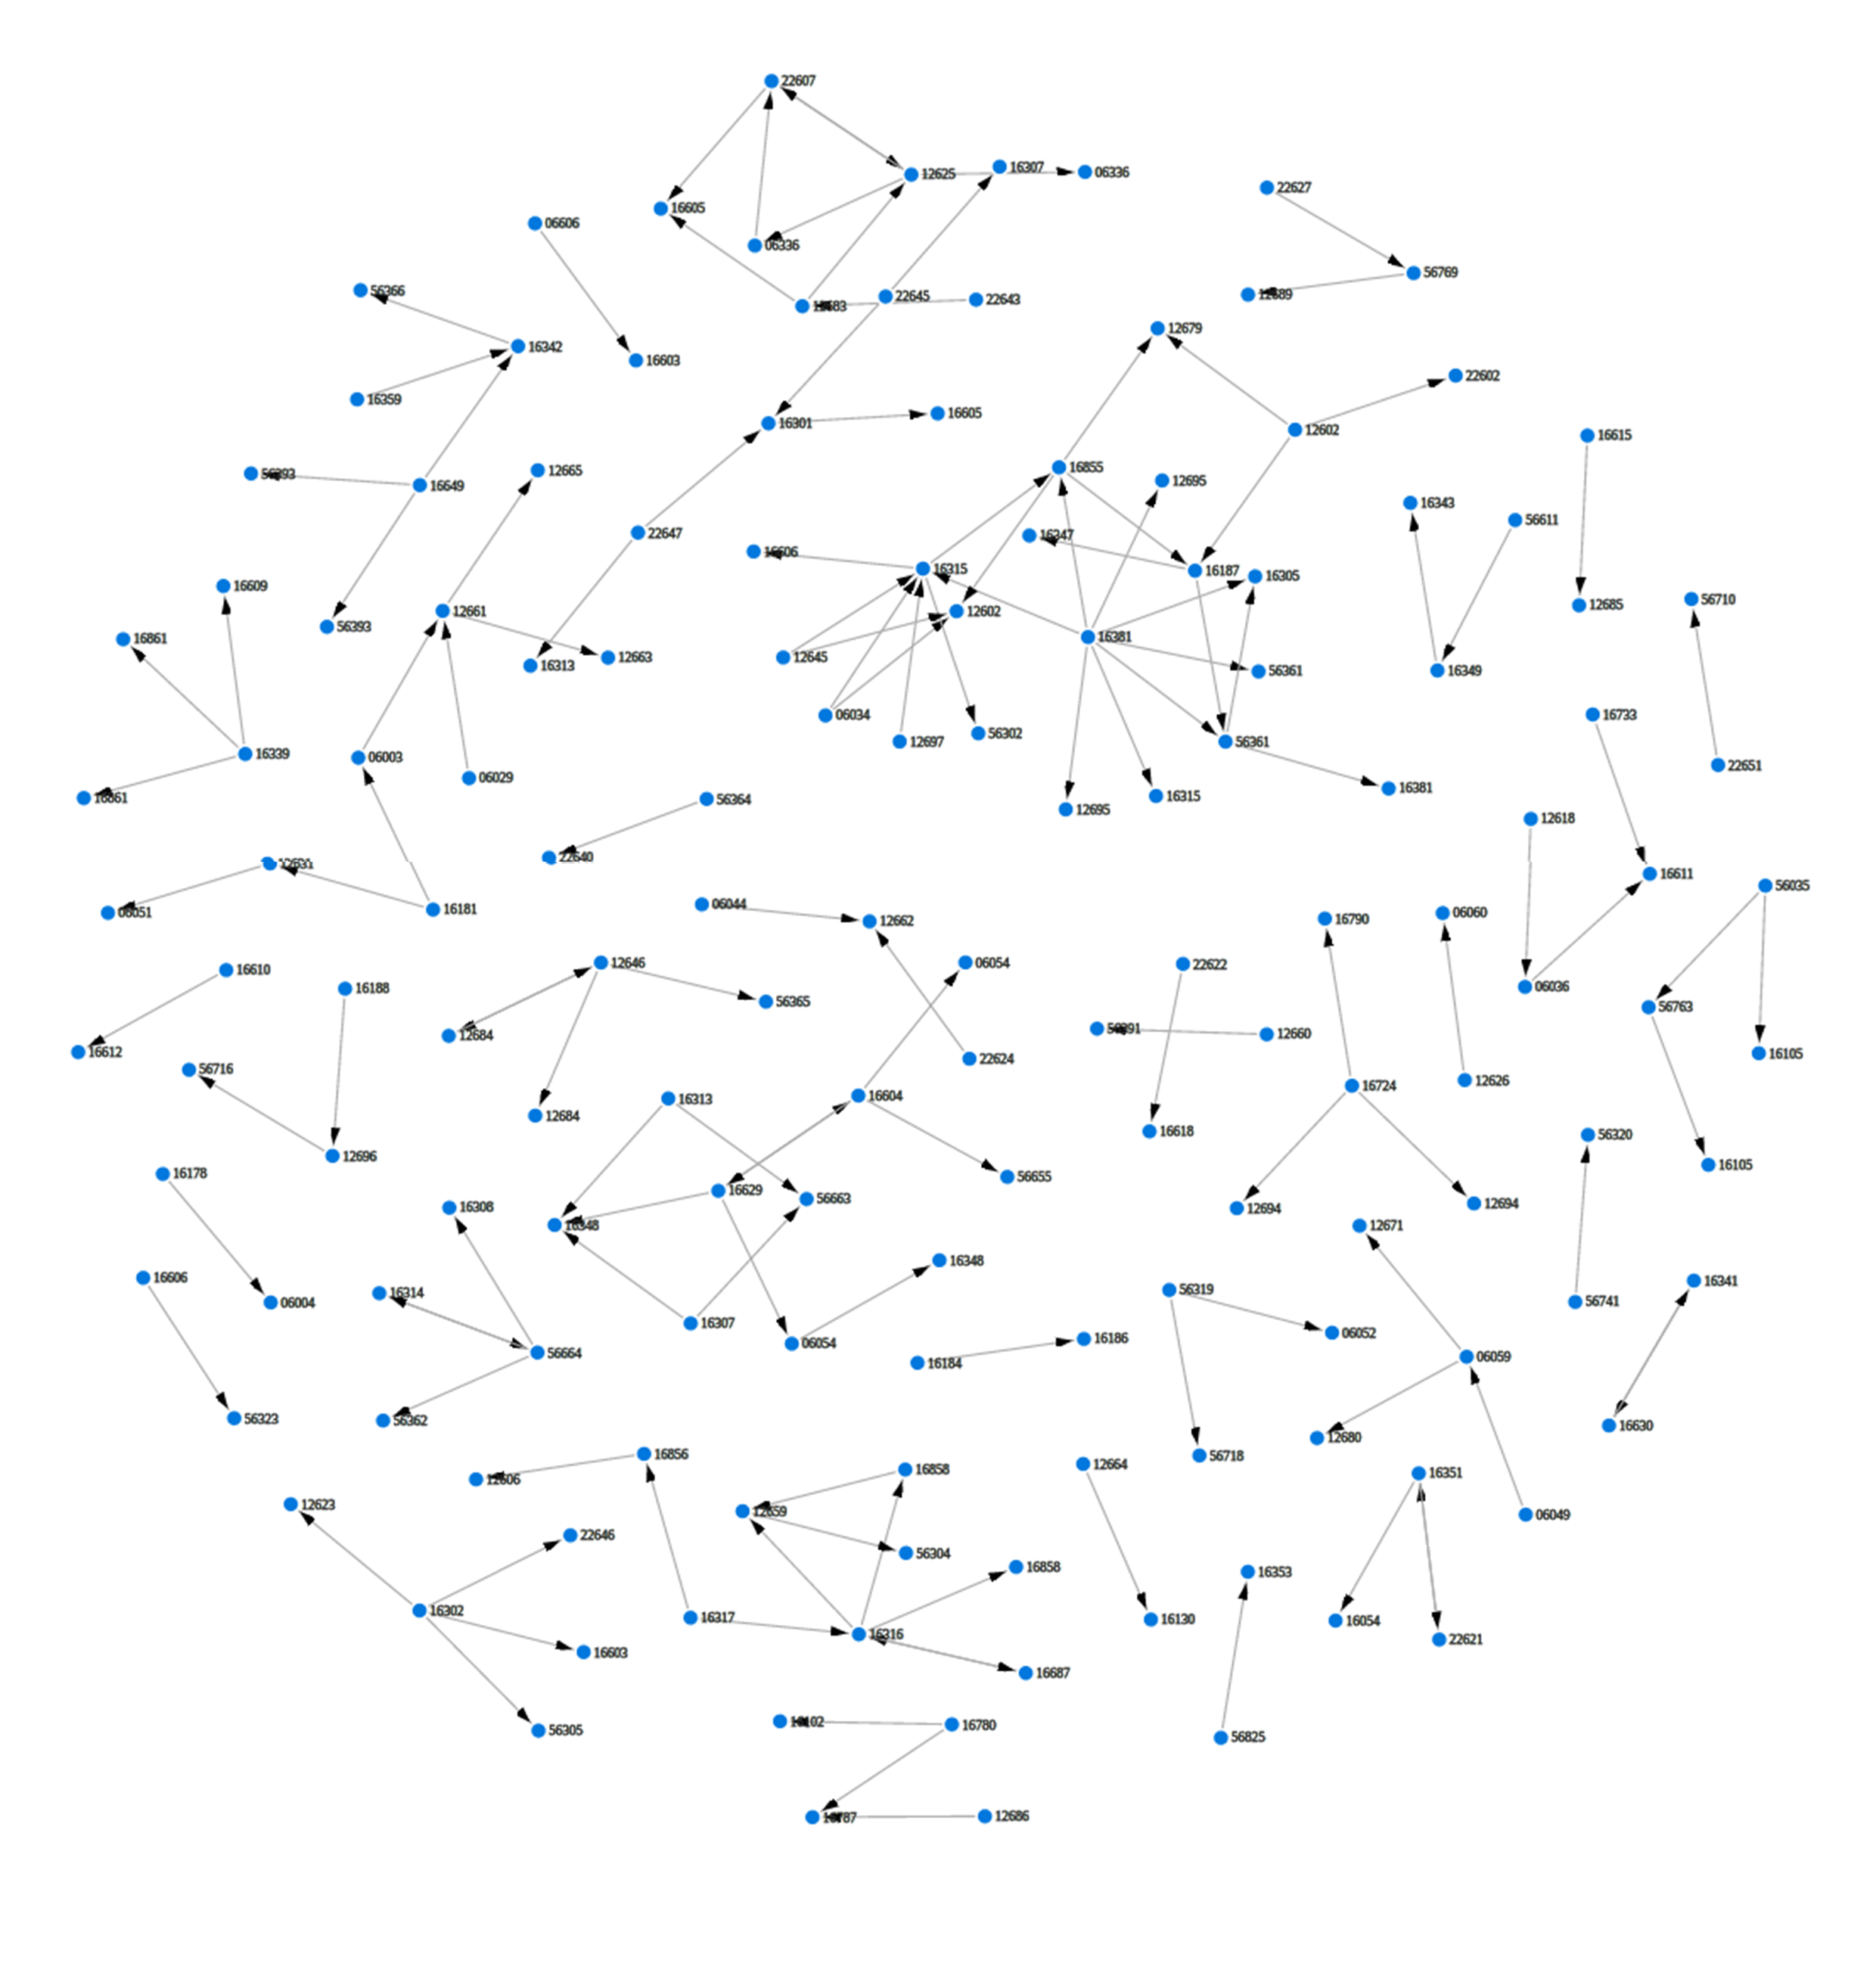
\includegraphics[scale=0.93]{img/train_delay_reason.png} \\
	\textbf{Figure 5:} visualization of the reason for a train delay ({\em for the Default run )} \\ {\em Directed edge $a \to b$ indicating $a$ is delayed due to $b$}\\
	
\end{center}
\end{changemargin}

\newpage

\section{Conclusion}

In this paper a Discrete Event Simulation Program is presented, that can basically evaluate the performance of a provided input static-schedule. The schedule is simulated over a modelled network using a semaphore signalling scheme as the underlying signalling protocol. This program would be useful to evaluate schedules and help in optimizing it if necessary. Though the presented simulator makes a crude approximate of the underlying complex interactions, it is a very powerful technique that can be extended to adapt to more complex models. Experimentally it is observed that the delays caused due to signalling and the way the static schedule is designed can be reduced by using the on-line randomized algorithm suggested by Leighton, Maggs and Rao. The introduced alternative algorithm Random Delay at Intermediate Nodes [RDIN] also provides a schedule that has lower end-to-end delays, but is not as effective as the randomized on-line algorithm of LMR. \\

\noindent \underline{\em Source code :}  \url{https://gitlab.iitm.ac.in/cs14b058/Railway-Network-Simulation} 

\section{Future Work}

The simulation model presented here is just a scratch on the surface of a plethora of things that can be considered as a simulation parameter. Railway operations being a complex interaction, modelling it exactly is near impossible. However with sufficient historic data of the operation simulation parameters can be derived for delays such as passenger boarding delay, weather conditions etc.,

\noindent The signalling in the railways is more complex as there are warning signals that ensure the train runs at a lower speed than the usual. These complex signalling mechanisms can also be modelled and implemented in the simulator.

\noindent Extraneous delay causing factors such as operational delays, equipment delay can also be modelled with the availability of historic data about such occurrences.

\noindent The throttling factor for modelling these parameters is the lack of availability of data. To overcome this one must develop some clever analytical approximations that can be incorporated with the existing simulation model to provide a better evaluation of the schedule input to the program.

% Acknowledgements should go at the end, before appendices and references

\acks{I would like to thank Prof. Narayanaswamy for all the guidance and enriching discussions regarding the project. Also, I would like to thank Prof. Krishna Sivalingam for helping to choose SimJava as the choice of Discrete Event Simulator, which made the work considerably easier than using Network simulator ns3.}

\nocite{SignallingTypes}
\nocite{SignallingImgs}
\nocite{DelayInTrains}
\nocite{7313186}
\vskip 0.2in

\bibliographystyle{unsrt}
\bibliography{bibiliography}

\end{document}
